\subsection{Módulos numéricos en punto fijo (práctica 5)}
\label{sec:numerico}

La red necesita ángulos, cosenos, potencias de un tono y distancias, y en la FPGA no hay punto flotante. La
tabla~\ref{tab:formatos} resume los formatos; cada bloque se comparó contra el valor exacto.

\begin{table}[!htb]
\centering\footnotesize
\caption{Formatos de punto fijo del proyecto.}
\label{tab:formatos}
\rowcolors{2}{SoftGray}{white}
\begin{tabularx}{\textwidth}{@{}>{\bfseries\raggedright\arraybackslash}p{3.2cm} >{\raggedright\arraybackslash}p{4.4cm} >{\raggedright\arraybackslash}X@{}}
\toprule
\rowcolor{TableHead} Magnitud & Formato & Resolución y razón \\
\midrule
Temperatura & 8 bits sin signo & 0.25~\textdegree C por cuenta, la del AMG8833 \\
Posición y distancia & 10 bits sin signo & 6.25~cm por cuenta sobre 64~m \\
Ángulo & 16 bits, un giro completo & 0.0055\textdegree{} por cuenta; el desbordamiento es el paso por 360\textdegree \\
CORDIC, $x$ e $y$ & 24 bits con signo y 4 de guarda & El redondeo queda por debajo de una cuenta \\
Coseno y seno & 18 bits, 14 de fracción & $2^{-14}=6.1\times10^{-5}$ \\
Goertzel & $c$ en Q2.14; estado de 18 bits & El estado no pasa de $2^{11}$ con 64 muestras \\
PID & Señales de 16 bits; ganancias Q8.8; integrador de 32 & $K_i\sum e$ sin truncar, con tope \\
\bottomrule
\end{tabularx}
\end{table}

\modulo{cordic}{hdl/cordic.v}{532 EL, 96 R}
\label{sec:cordic}%
Gira un vector por ángulos cada vez menores, de modo que cada giro se haga con sumas y
corrimientos~\cite{volder1959,andraka1998}:
\begin{equation}
x_{i+1}=x_i-d_i\,y_i\,2^{-i},\qquad y_{i+1}=y_i+d_i\,x_i\,2^{-i},\qquad z_{i+1}=z_i-d_i\arctan 2^{-i},
\end{equation}
con $d_i=\pm1$. Es secuencial, una iteración por ciclo, con una tabla de arcotangentes y sin multiplicadores. En
\textbf{rotación} lleva $z$ a cero: con $(1/K,0)$ entrega $(\cos z_0,\sin z_0)$, que usa la triangulación. En
\textbf{vectorización} lleva $y$ a cero: entrega $\operatorname{atan2}(y_0,x_0)$ y la magnitud por
$K=1.646760$; lo usa el sensor simulado. Antes de iterar lleva el problema al semiplano derecho con un giro de
180\textdegree, porque solo converge para $\pm99.9$\textdegree. Latencia: $N+2$ ciclos (figura~\ref{fig:rtlcordic}).

\begin{figure}[!htb]
\centering
\begin{subfigure}{\textwidth}
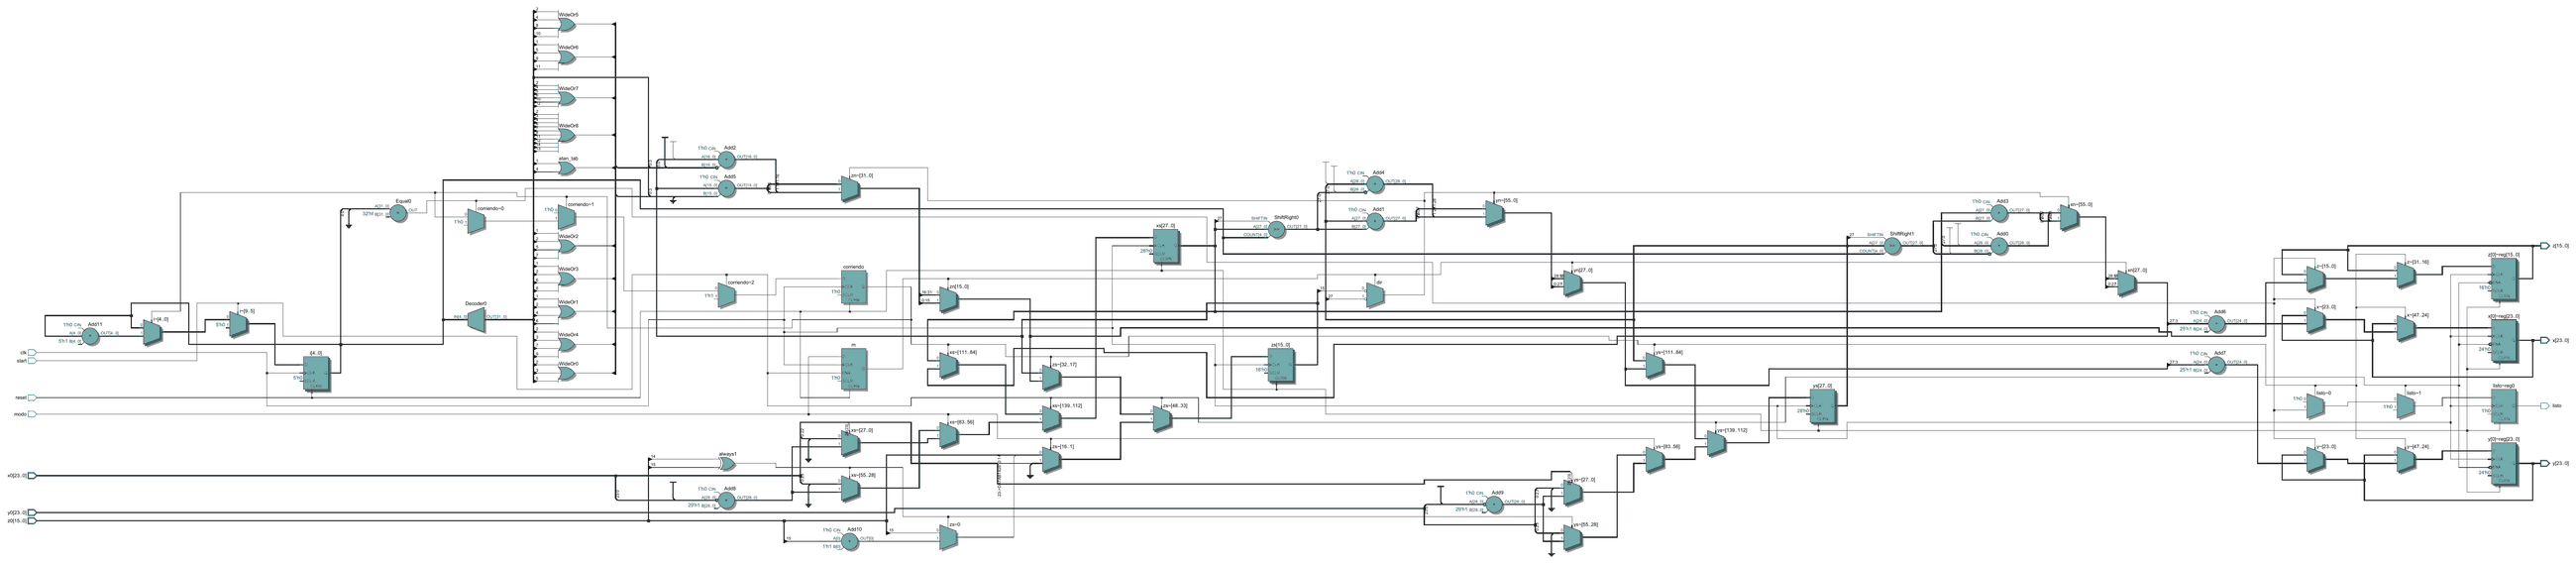
\includegraphics[width=\linewidth]{figs/rtl/rtl_cordic.png}
\caption{El módulo completo; a la izquierda, la tabla de arcotangentes.}
\end{subfigure}

\medskip
\begin{subfigure}{0.52\textwidth}
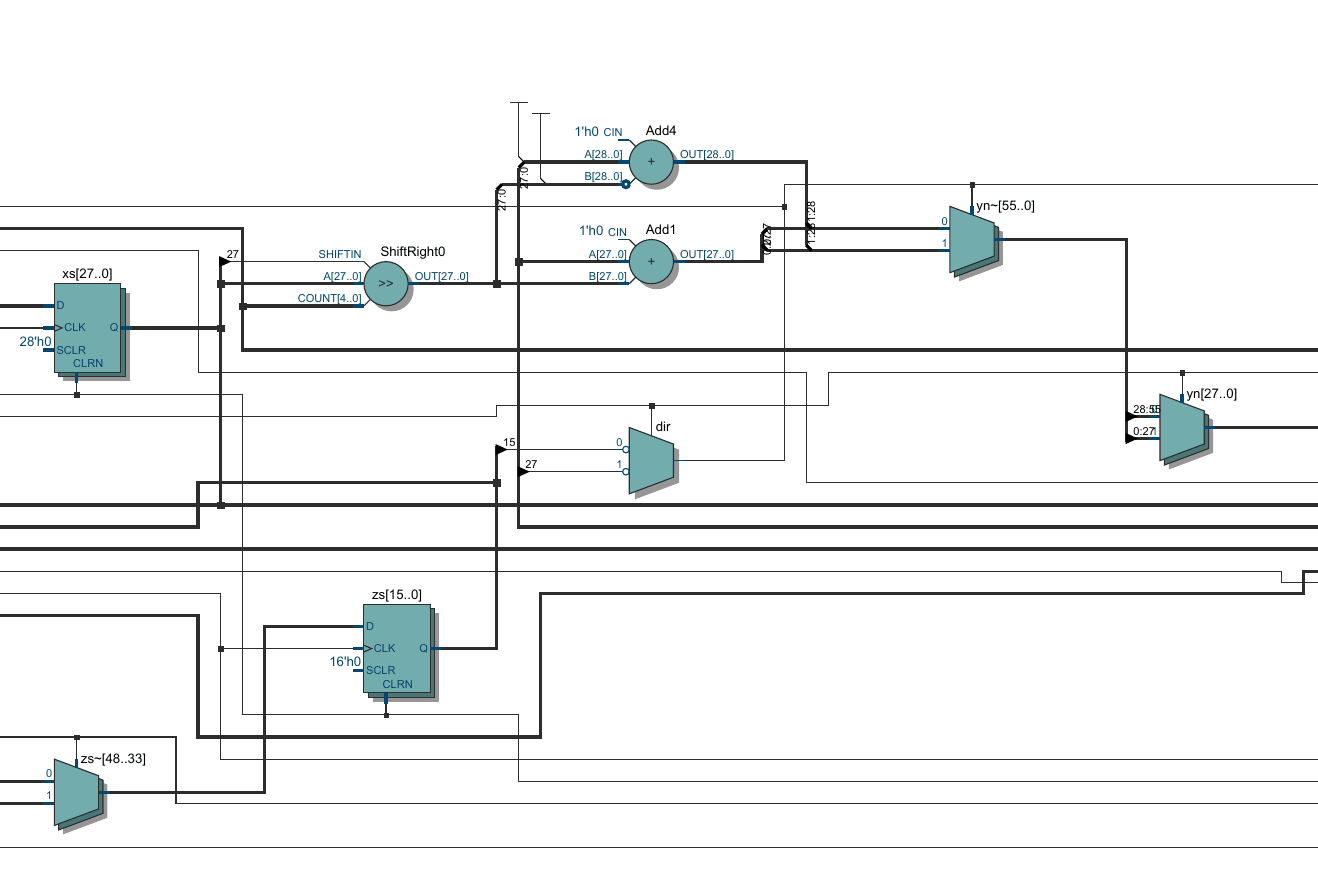
\includegraphics[width=\linewidth]{figs/rtl/zoom_cordic.png}
\caption{Acercamiento a una iteración: corrimiento de $x$, suma y resta, y el sentido de giro \sig{dir}.}
\end{subfigure}
\caption{\sig{cordic} en el RTL Viewer.}
\label{fig:rtlcordic}
\end{figure}

Nueve circuitos iguales, con $N$ de 4 a 20, recibieron los mismos 360 vectores y 360 ángulos
(figura~\ref{fig:cordiciter} y tabla~\ref{tab:cordiciter}). El error se divide entre cuatro cada dos iteraciones
hasta $N=14$ y ahí se estanca, porque la tabla de 16 bits se agota. Con $N=16$ el error máximo es de
0.017\textdegree, veinte veces menos que el paso de 0.35\textdegree{} con que el rumbo viaja por la red.
\sig{tb\_cordic} prueba además los cuatro cuadrantes y 200 divisiones: 248 de 248.

\begin{figure}[!htb]
\centering
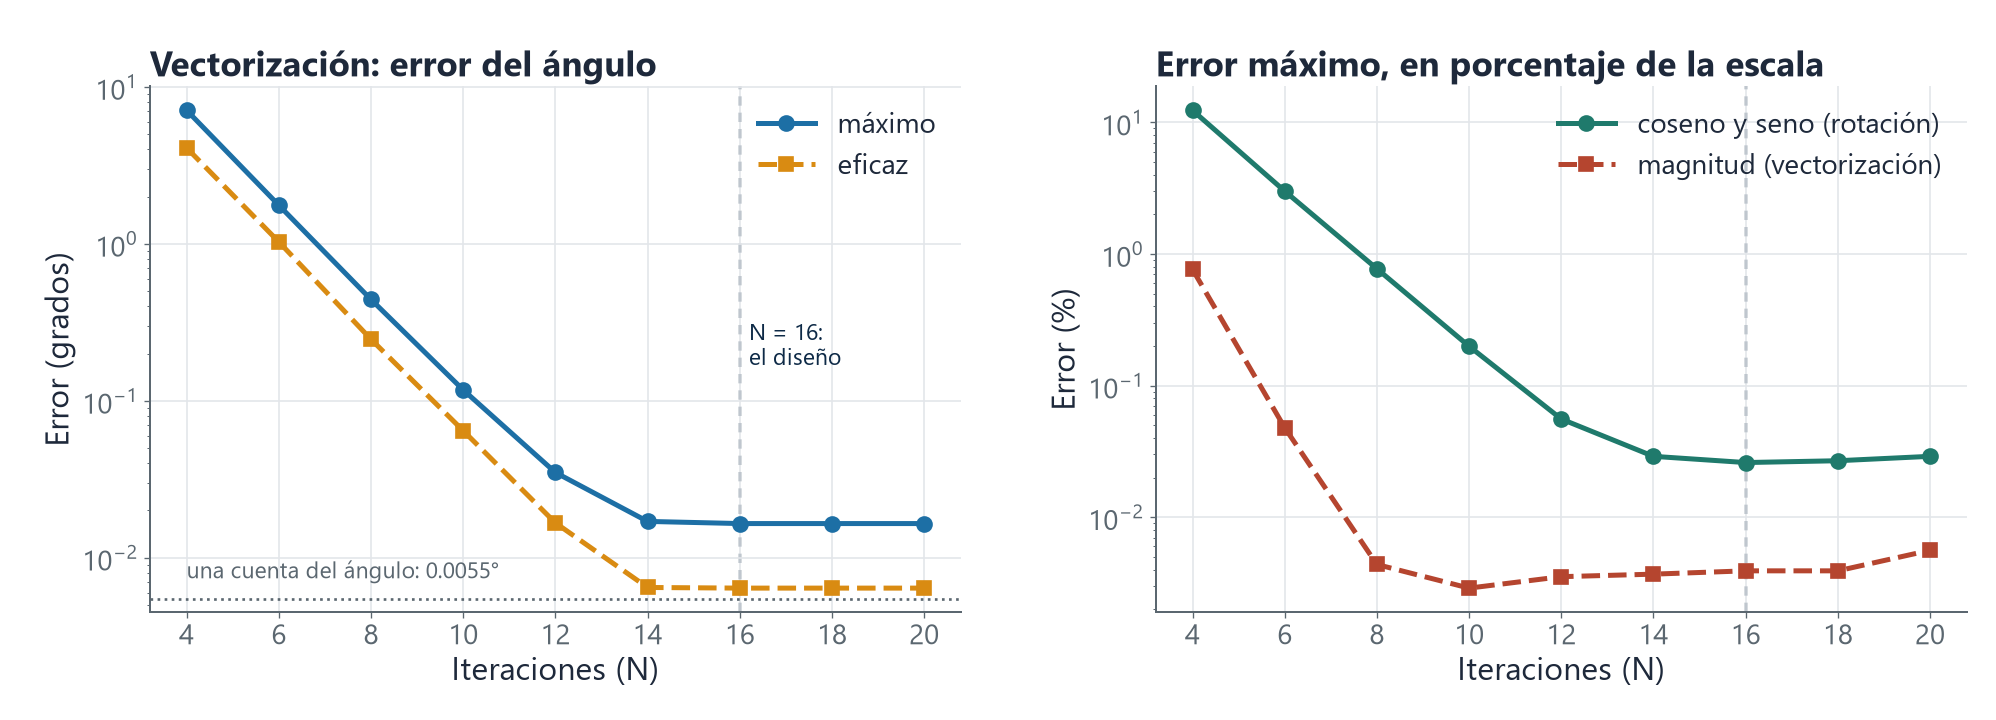
\includegraphics[width=0.96\textwidth]{figs/cordic_iteraciones.png}
\caption{Error del CORDIC según el número de iteraciones, medido en la simulación del circuito.}
\label{fig:cordiciter}
\end{figure}

\begin{table}[!htb]
\centering\footnotesize
\caption{Error máximo del CORDIC (\sig{tb\_cordic\_iter}).}
\label{tab:cordiciter}
\rowcolors{2}{SoftGray}{white}
\begin{tabularx}{0.86\textwidth}{@{}>{\bfseries}c >{\raggedleft\arraybackslash}X >{\raggedleft\arraybackslash}X >{\raggedleft\arraybackslash}X >{\raggedleft\arraybackslash}X@{}}
\toprule
\rowcolor{TableHead} $N$ & Ángulo (\textdegree) & Ángulo, eficaz (\textdegree) & Magnitud (\%) & Coseno y seno (\%) \\
\midrule
4  & 7.093 & 4.083 & 0.764 & 12.369 \\
8  & 0.442 & 0.246 & 0.0044 & 0.773 \\
12 & 0.035 & 0.017 & 0.0035 & 0.056 \\
16 & 0.017 & 0.0064 & 0.0039 & 0.026 \\
20 & 0.017 & 0.0064 & 0.0056 & 0.029 \\
\bottomrule
\end{tabularx}
\end{table}

\modulo{divisor\_u}{hdl/cordic.v}{84 a 195 EL}
Divisor con restauración: por ciclo baja un bit del dividendo al resto, prueba si cabe el divisor y, si cabe, lo
resta y pone un 1 en el cociente. Tarda un ciclo por bit más uno. La triangulación usa uno de 44 entre 32 bits y
el rumbo, uno de 20 entre 7.

\modulo{tri\_distancia}{hdl/tri\_red.v}{87 a 109 EL, 60 R}
\label{sec:raiz}%
Calcula $d=\lfloor\sqrt{\Delta x^2+\Delta y^2}\rfloor$ con la raíz dígito por dígito: baja dos bits del radicando
de 22 por ciclo, prueba si cabe $4q+1$ en el resto y, si cabe, lo resta y agrega un 1 a la raíz. En 12 ciclos da la
parte entera exacta. La regla del alcance usa la misma suma de cuadrados, $\Delta x^2+\Delta y^2<(16\times32)^2$,
así que la distancia que se muestra y el corte de los 32~m no pueden contradecirse (figura~\ref{fig:rtldist}).

\begin{figure}[!htb]
\centering
\begin{subfigure}{\textwidth}
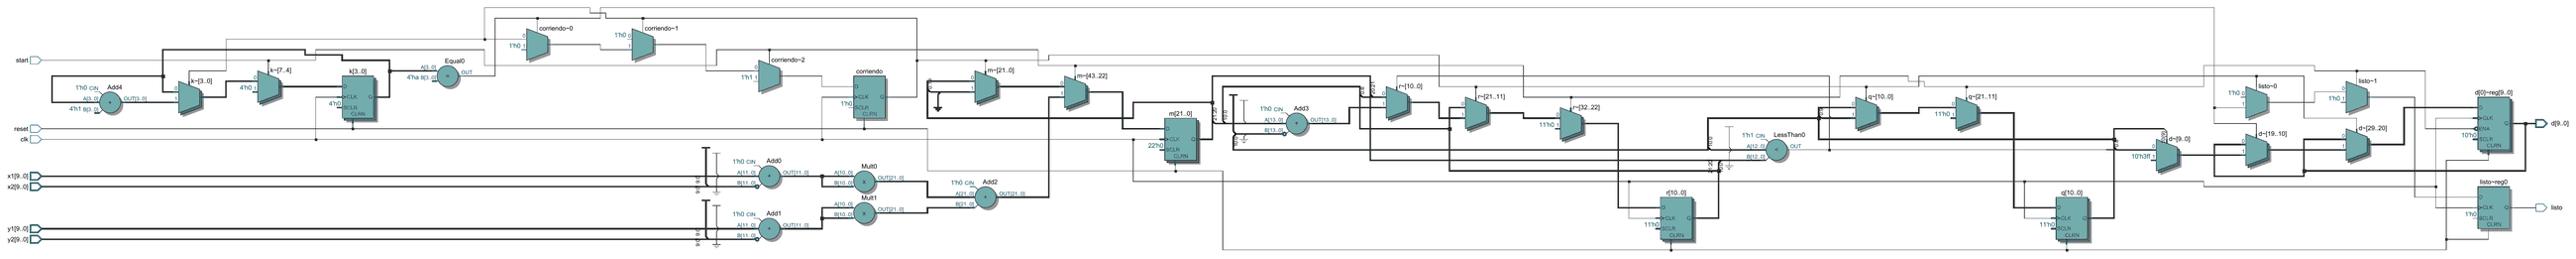
\includegraphics[width=\linewidth]{figs/rtl/rtl_tri_distancia.png}
\caption{El módulo completo.}
\end{subfigure}

\medskip
\begin{subfigure}{0.86\textwidth}
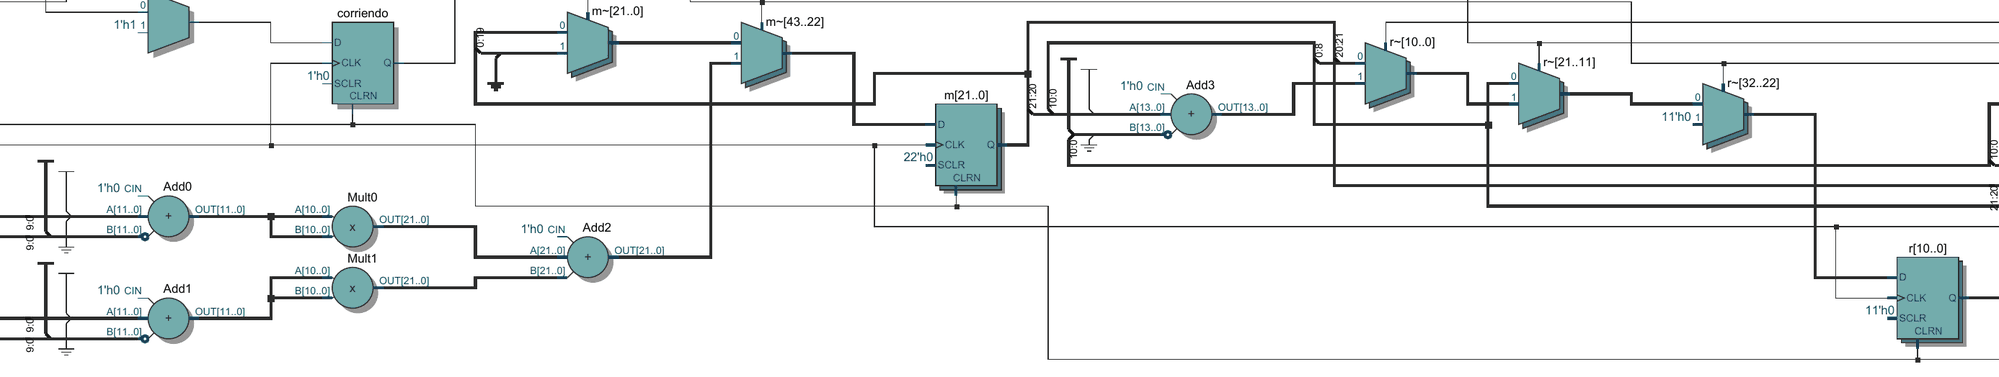
\includegraphics[width=\linewidth]{figs/rtl/zoom_tri_distancia.png}
\caption{Acercamiento: restas, los dos cuadrados (\sig{Mult0} y \sig{Mult1}), su suma y el registro del radicando.}
\end{subfigure}
\caption{\sig{tri\_distancia} en el RTL Viewer.}
\label{fig:rtldist}
\end{figure}

\textbf{FIR: media móvil.}\phantomsection\label{sec:fir} El filtro del núcleo es
$y[n]=\tfrac14(x[n]+x[n-1]+x[n-2]+x[n-3])$. No tiene realimentación, así que es estable, y su fase es lineal:
retrasa la señal un cuadro y medio sin deformarla. Con diez cuadros por segundo tiene nulos en 2.5 y 5~Hz
(figura~\ref{fig:filtros}, izquierda).

\modulo{tri\_tonos}{hdl/tonos.v}{355 EL, 225 R}
\label{sec:goertzel}%
Cada nodo emite un tono propio y escucha los otros dos: con saber a quién oye, sabe quién está a su alcance. El
micrófono, simulado como la suma de las ondas cuadradas que llegan más ruido, se muestrea a 16~kHz y cada 64
muestras (4~ms) tres filtros de Goertzel~\cite{goertzel1958} miden la potencia:
\begin{equation}
s[n]=x[n]+c\,s[n-1]-s[n-2],\qquad P=s[N_b-1]^2+s[N_b-2]^2-c\,s[N_b-1]\,s[N_b-2],
\end{equation}
con $c=2\cos(2\pi k/N_b)$. Los tonos de 1, 2 y 4~kHz caen en las líneas $k=4$, 8 y 16, de modo que uno no se cuela
en el filtro de otro; los coeficientes son 30\,274, 23\,170 y 0 en Q2.14. Un IIR con polos sobre el círculo
unitario podría acumular error, pero este corre 64 muestras y borra su estado. Un tono se da por oído si su
potencia pasa de 4\,000 en dos bloques seguidos y por perdido si queda debajo en dos: con el tono presente mide de
27\,000 a 33\,000 y sin él no pasa de 104 (figura~\ref{fig:filtros}, derecha). El tono propio sale por el pin~1 de
JP1, listo para un zumbador; con un micrófono real solo se sustituye la suma simulada.

\begin{figure}[!htb]
\centering
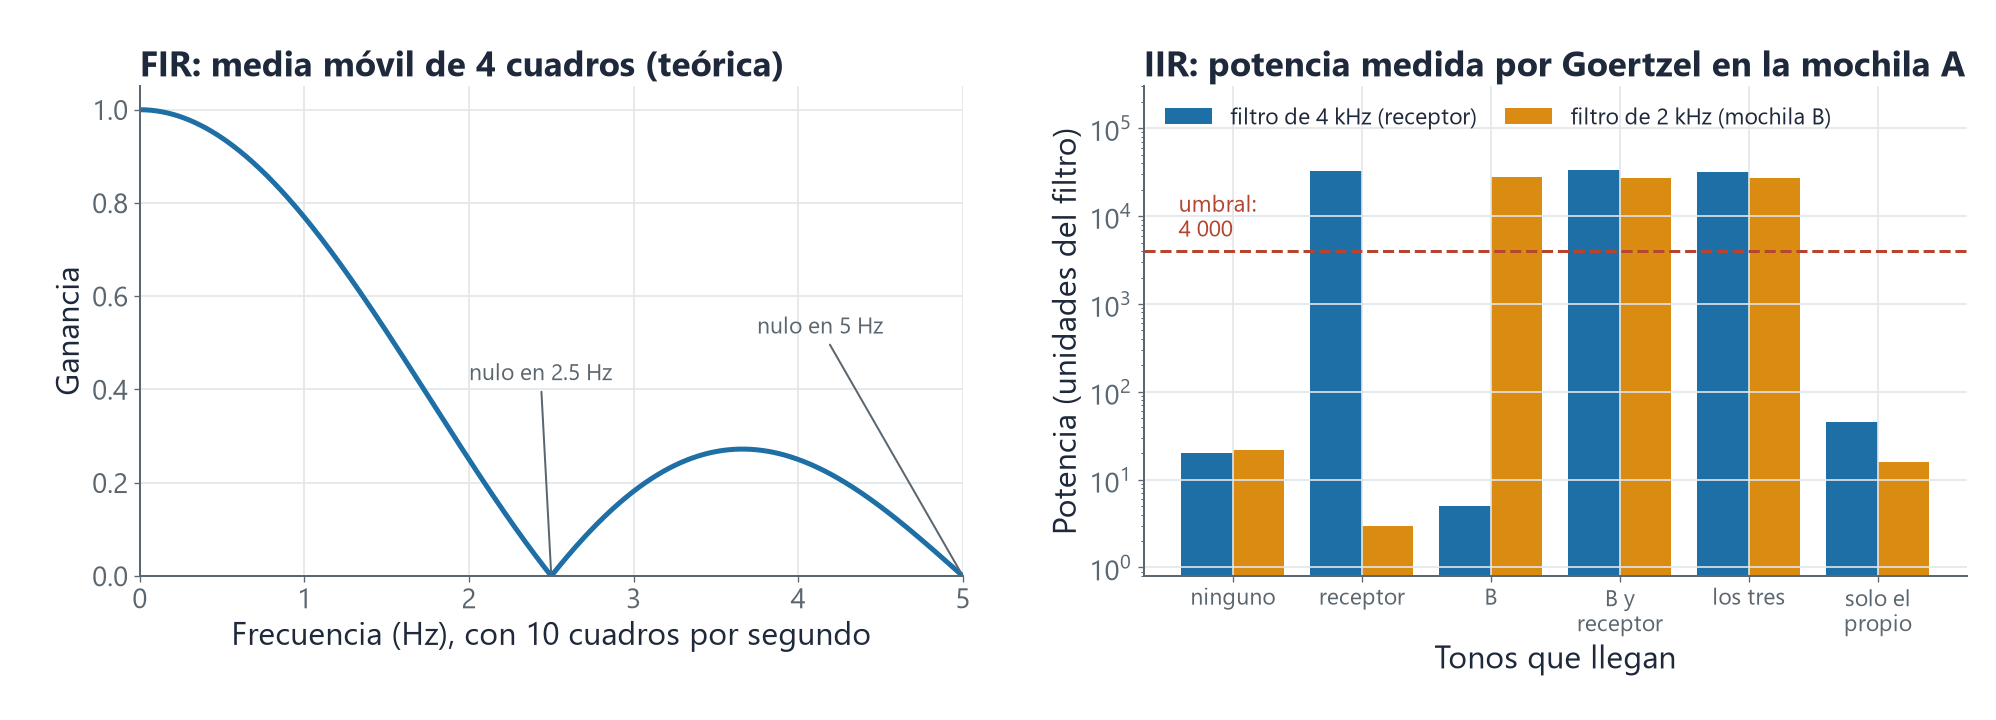
\includegraphics[width=0.97\textwidth]{figs/filtros.png}
\caption{Izquierda: respuesta de la media móvil (curva teórica). Derecha: potencia medida por los filtros de
Goertzel de la mochila A en la simulación del circuito (\sig{tb\_tonos}).}
\label{fig:filtros}
\end{figure}

\modulo{pid\_q}{hdl/pid\_q.v}{213 EL, 66 R, 79.96 MHz}
\label{sec:pid}%
PID en forma posicional, una muestra por pulso:
\begin{equation}
e[n]=r[n]-y[n],\qquad u[n]=K_p\,e[n]+K_i\sum_{k\le n}e[k]+K_d\,\bigl(e[n]-e[n-1]\bigr).
\end{equation}
El integral es un acumulador de 32 bits que guarda $K_i\sum e$ con sus ocho bits de fracción. La salida se satura
en $\pm U_{\max}$ y la saturación se decide con la suma completa de 40 bits. Si el actuador está en el tope y el
error empuja hacia el mismo lado, el acumulador se congela (integración condicional); un parámetro quita la
protección para compararla (figura~\ref{fig:rtlpid}). \sig{tb\_pid} cierra el lazo sobre $y[n+1]=y[n]+(4u[n]-y[n])/20$ junto a un PID en
aritmética real (figura~\ref{fig:pid}): la salida difiere en menos de una cuenta. El escalón de 200 tiene 9.3~\% de
sobrepaso y entra al 2~\% en 49 muestras; el de 1\,000, con el actuador saturado, 0.2~\% y 66 muestras, mientras
que sin protección la salida sigue en el tope 400 muestras después.

\begin{figure}[!htb]
\centering
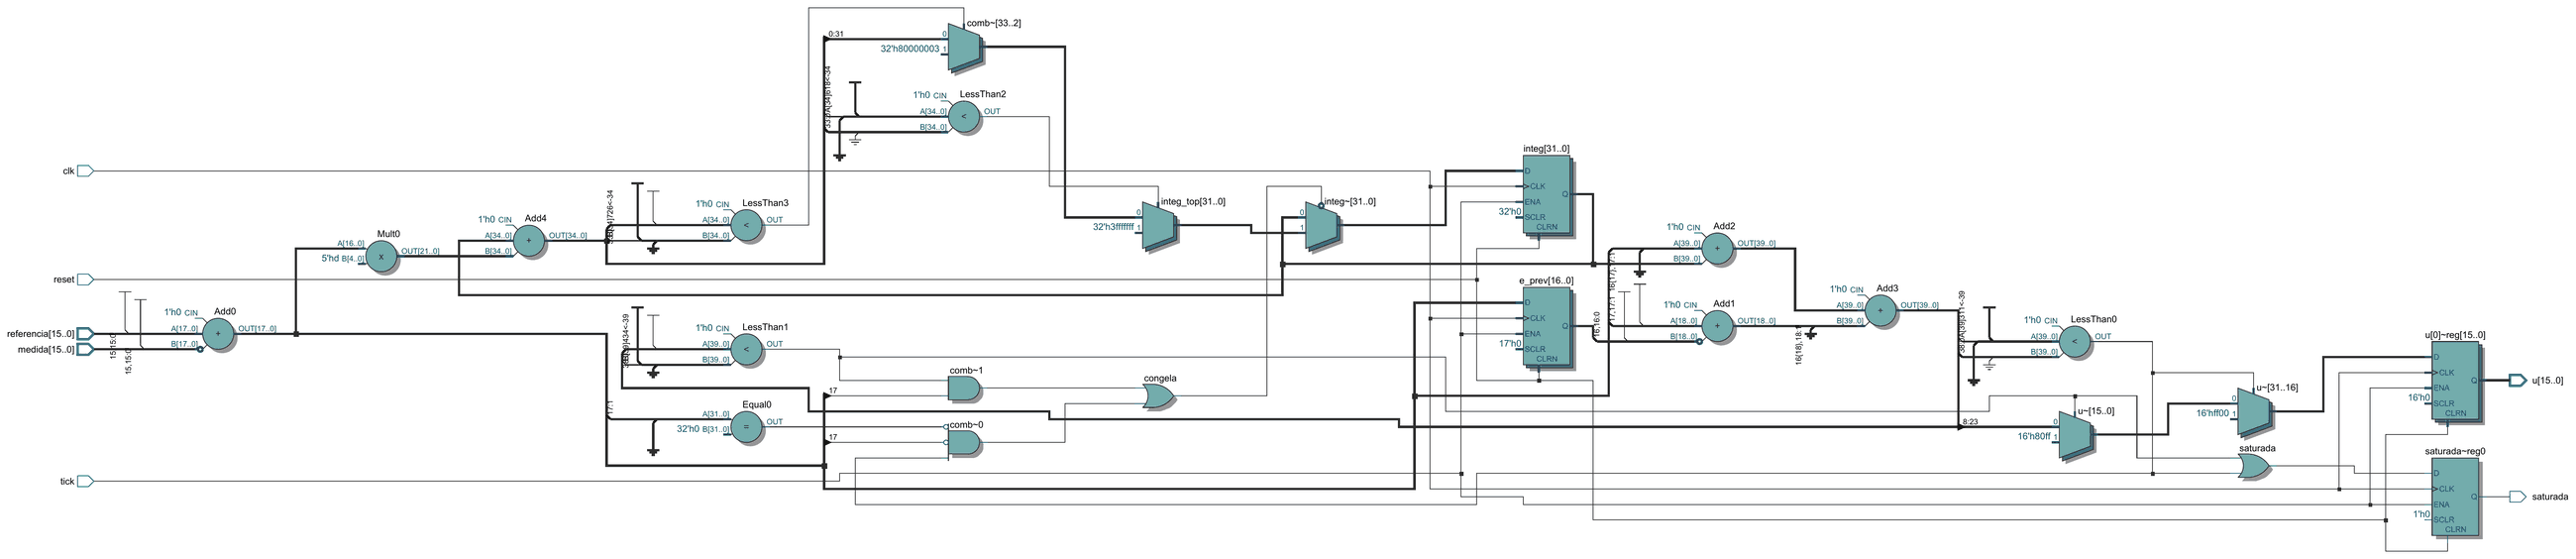
\includegraphics[width=\textwidth]{figs/rtl/rtl_pid_q.png}
\caption{\sig{pid\_q} en el RTL Viewer: error, producto integral, integrador con tope, congelamiento (\sig{congela}) y
saturación de la salida.}
\label{fig:rtlpid}
\end{figure}

\begin{figure}[!htb]
\centering
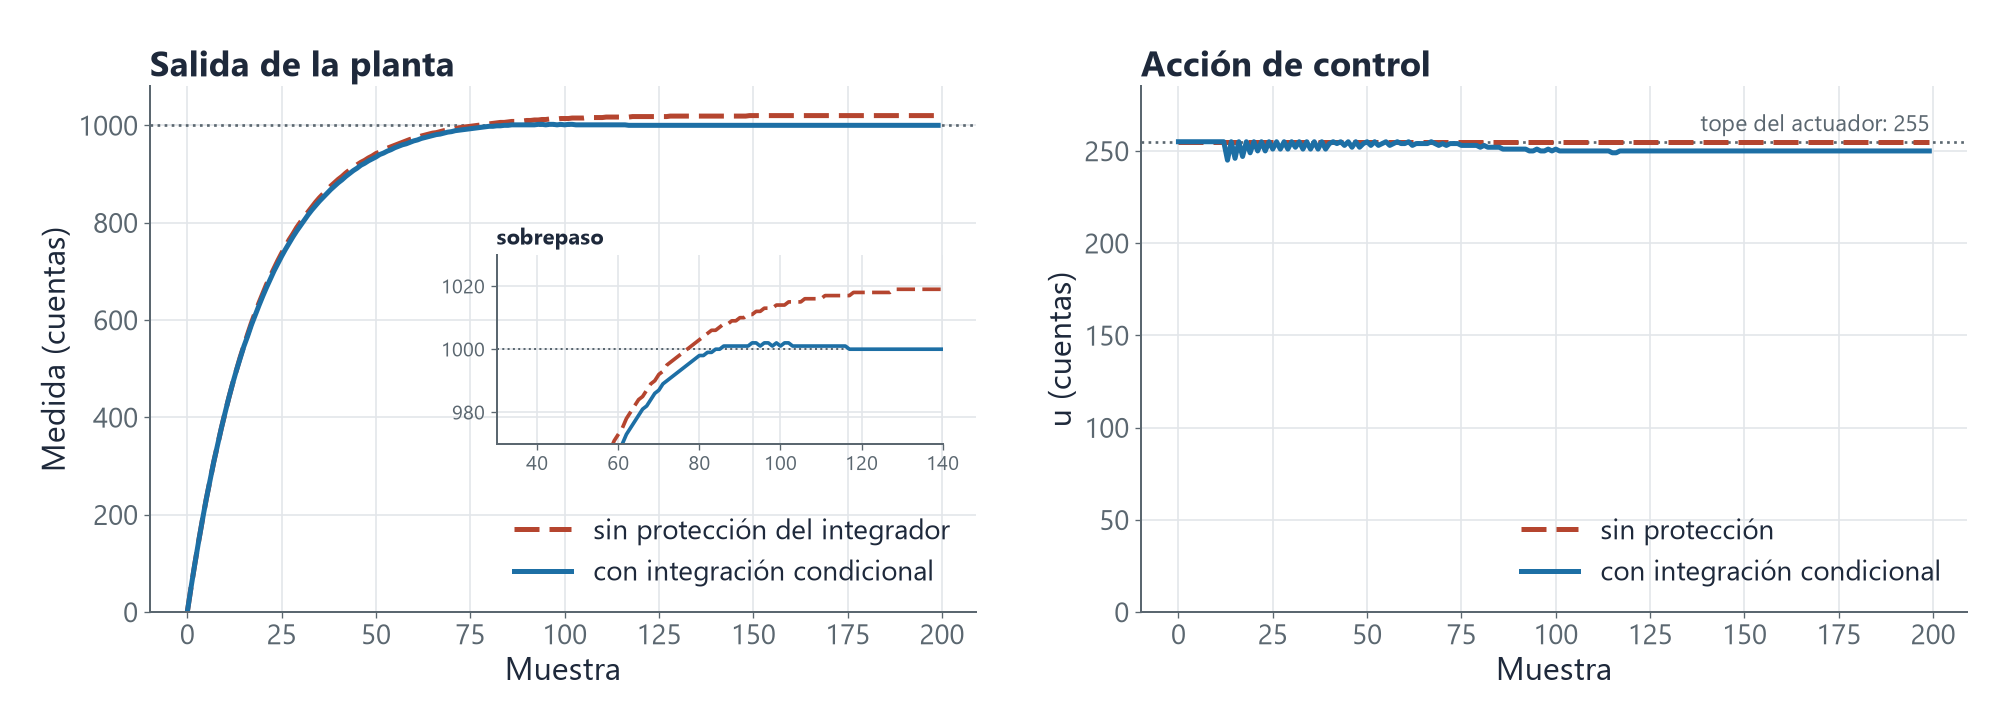
\includegraphics[width=0.86\textwidth]{figs/pid_respuesta.png}
\caption{Escalón de 1\,000 con el actuador saturado. Sin protección, la planta no vuelve a la referencia.}
\label{fig:pid}
\end{figure}

La búsqueda no usa un PID, porque su actuador es un pulso que el insecto obedece o no. Corresponde al modo de
regreso (sección~\ref{sec:regreso}): llevar a cero la diferencia entre dos fotodiodos que miran al faro, con la
tasa de estímulos como actuador. Ese modo no está en la demostración; aquí queda verificado con una planta de
prueba.
